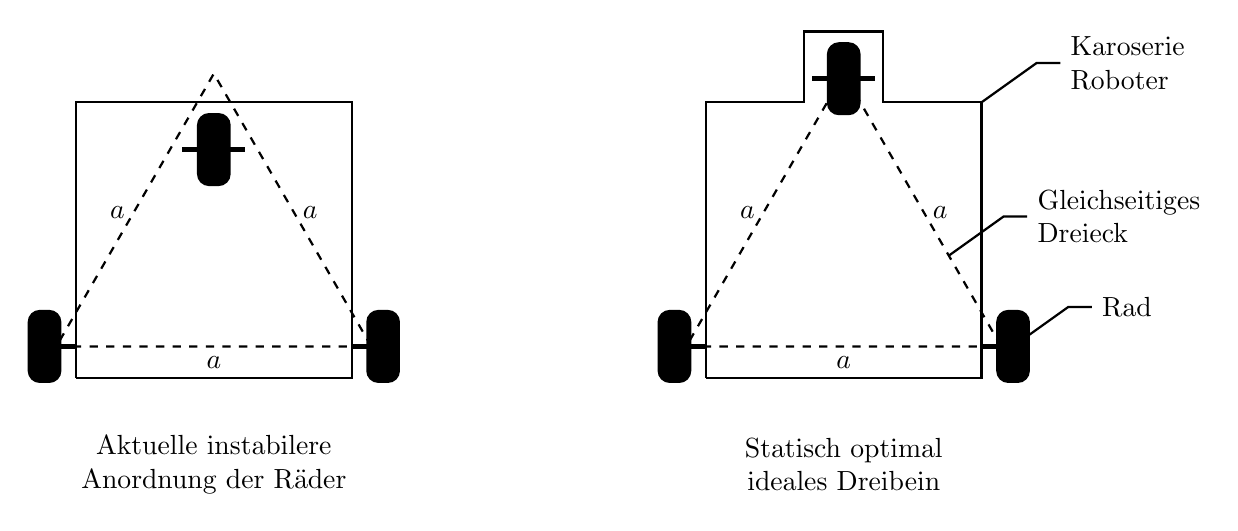
\begin{tikzpicture}[thick]
	

			\begin{scope}[shift={(0,0)}]
			
			% Punkte
			\coordinate (A) at (0,0);
			\coordinate (B) at (4,0);
			\coordinate (C) at (2,{2*sqrt(3)});
			
			% Dreieck
			\draw[dashed, dash pattern=on 3pt off 3pt] (A) -- (B) -- (C) -- cycle;
			
			\draw[thick] (0.25,-0.4) -- ++ (3.5,0) -- ++ (0,3.5) -- ++ (-3.5,0) -- ++ (0,-3.5);
			% Beschriftung
%			\node[below left]  at (A) {A};
%			\node[below right] at (B) {B};
%			\node[above]       at (C) {C};
			
		% Seiten
		\node[below] at (2,0) {$a$};
		\node[left]  at (1,1.7) {$a$};
		\node[right] at (3,1.7) {$a$};
			
			%Reifen links
			\draw[rounded corners,fill=black]
			(0.25-0.6,+0.45) rectangle (0.25-0.2,-0.45);
			\draw[line width=2] (0.25,0) -- ++ (-0.2,0);
			%Reifen Rechts
			\draw[rounded corners,fill=black]
			(3.75+0.6,+0.45) rectangle (3.75+0.2,-0.45);
			\draw[line width=2] (3.75,0) -- ++ (+0.2,0);
			
			Einzelnes Rad
			\draw[rounded corners,fill=black]
			(2-0.2,2.5+0.45) rectangle (2+0.2,2.5-0.45);
			\draw[line width=2] (2-0.4,2.5) -- ++ (+0.8,0);
			
			\node[align=center]  at (2,-1.5) {Aktuelle instabilere\\Anordnung der Räder};
		\end{scope}
		
		
		\begin{scope}[shift={(8,0)}]
	
		% Punkte
		\coordinate (A) at (0,0);
		\coordinate (B) at (4,0);
		\coordinate (C) at (2,{2*sqrt(3)});
		
		% Dreieck
		\draw[dashed, dash pattern=on 3pt off 3pt] (A) -- (B) -- (C) -- cycle;
		
		\draw[thick] (0.25,-0.4) -- ++ (0,3.5) -- (0.25+1.25,-0.4+3.5) -- ++ (0,0.9) -- ++ (1,0) -- ++ (0,-0.9) -- (0.25+3.5,-0.4+3.5) -- ++ (0,-3.5) -- ++ (-3.5,0);
		
		\draw[] (0.25+1.25,-0.4+3.5) -- ++ (0,0.9) -- ++ (1,0) -- ++ (0,-0.9);
		% Beschriftung
%		\node[below left]  at (A) {A};
%		\node[below right] at (B) {B};
%		\node[above]       at (C) {C};
		
		% Seiten
		\node[below] at (2,0) {$a$};
		\node[left]  at (1,1.7) {$a$};
		\node[right] at (3,1.7) {$a$};
	
		%Reifen links
		\draw[rounded corners,fill=black]
		(0.25-0.6,+0.45) rectangle (0.25-0.2,-0.45);
		\draw[line width=2] (0.25,0) -- ++ (-0.2,0);
		%Reifen Rechts
		\draw[rounded corners,fill=black]
		(3.75+0.6,+0.45) rectangle (3.75+0.2,-0.45);
		\draw[line width=2] (3.75,0) -- ++ (+0.2,0);
	
		Einzelnes Rad
						\draw[rounded corners,fill=black]
						(2-0.2,3.4+0.45) rectangle (2+0.2,3.4-0.45);
						\draw[line width=2] (2-0.4,3.4) -- ++ (+0.8,0);
						
			\node[align=center] at (2,-1.5) {Statisch optimal\\ideales Dreibein};
			
			\draw (3.75+0.4,0) -- ++ (0.7,0.5)  -- ++ (0.3,0) node[right] {Rad};
			\draw (3.75,3.1) -- ++ (0.7,0.5) -- ++ (0.3,0)
			node[right, align=left] {Karoserie\\Roboter};
			\draw (3.33,1.15) -- ++ (0.7,0.5)  -- ++ (0.3,0) node[right, align=left] {Gleichseitiges\\Dreieck};
		\end{scope}
	
\end{tikzpicture}